\subsection{Training on a balanced GENIE Dataset and evaluated on GiBUU Data}

\noindent In order to see if there was a bias in the training process the model previously described in the previous section was used to classify GiBUU events. As the model had previously been trained on GENIE only events, if the classification results of GiBUU were poorer, we could establish that the model had become too specific to GENIE dataset and that there were differences in how the GENIE and GiBUU simulated these events. \medskip

\begin{figure}[t!]
 \centering
 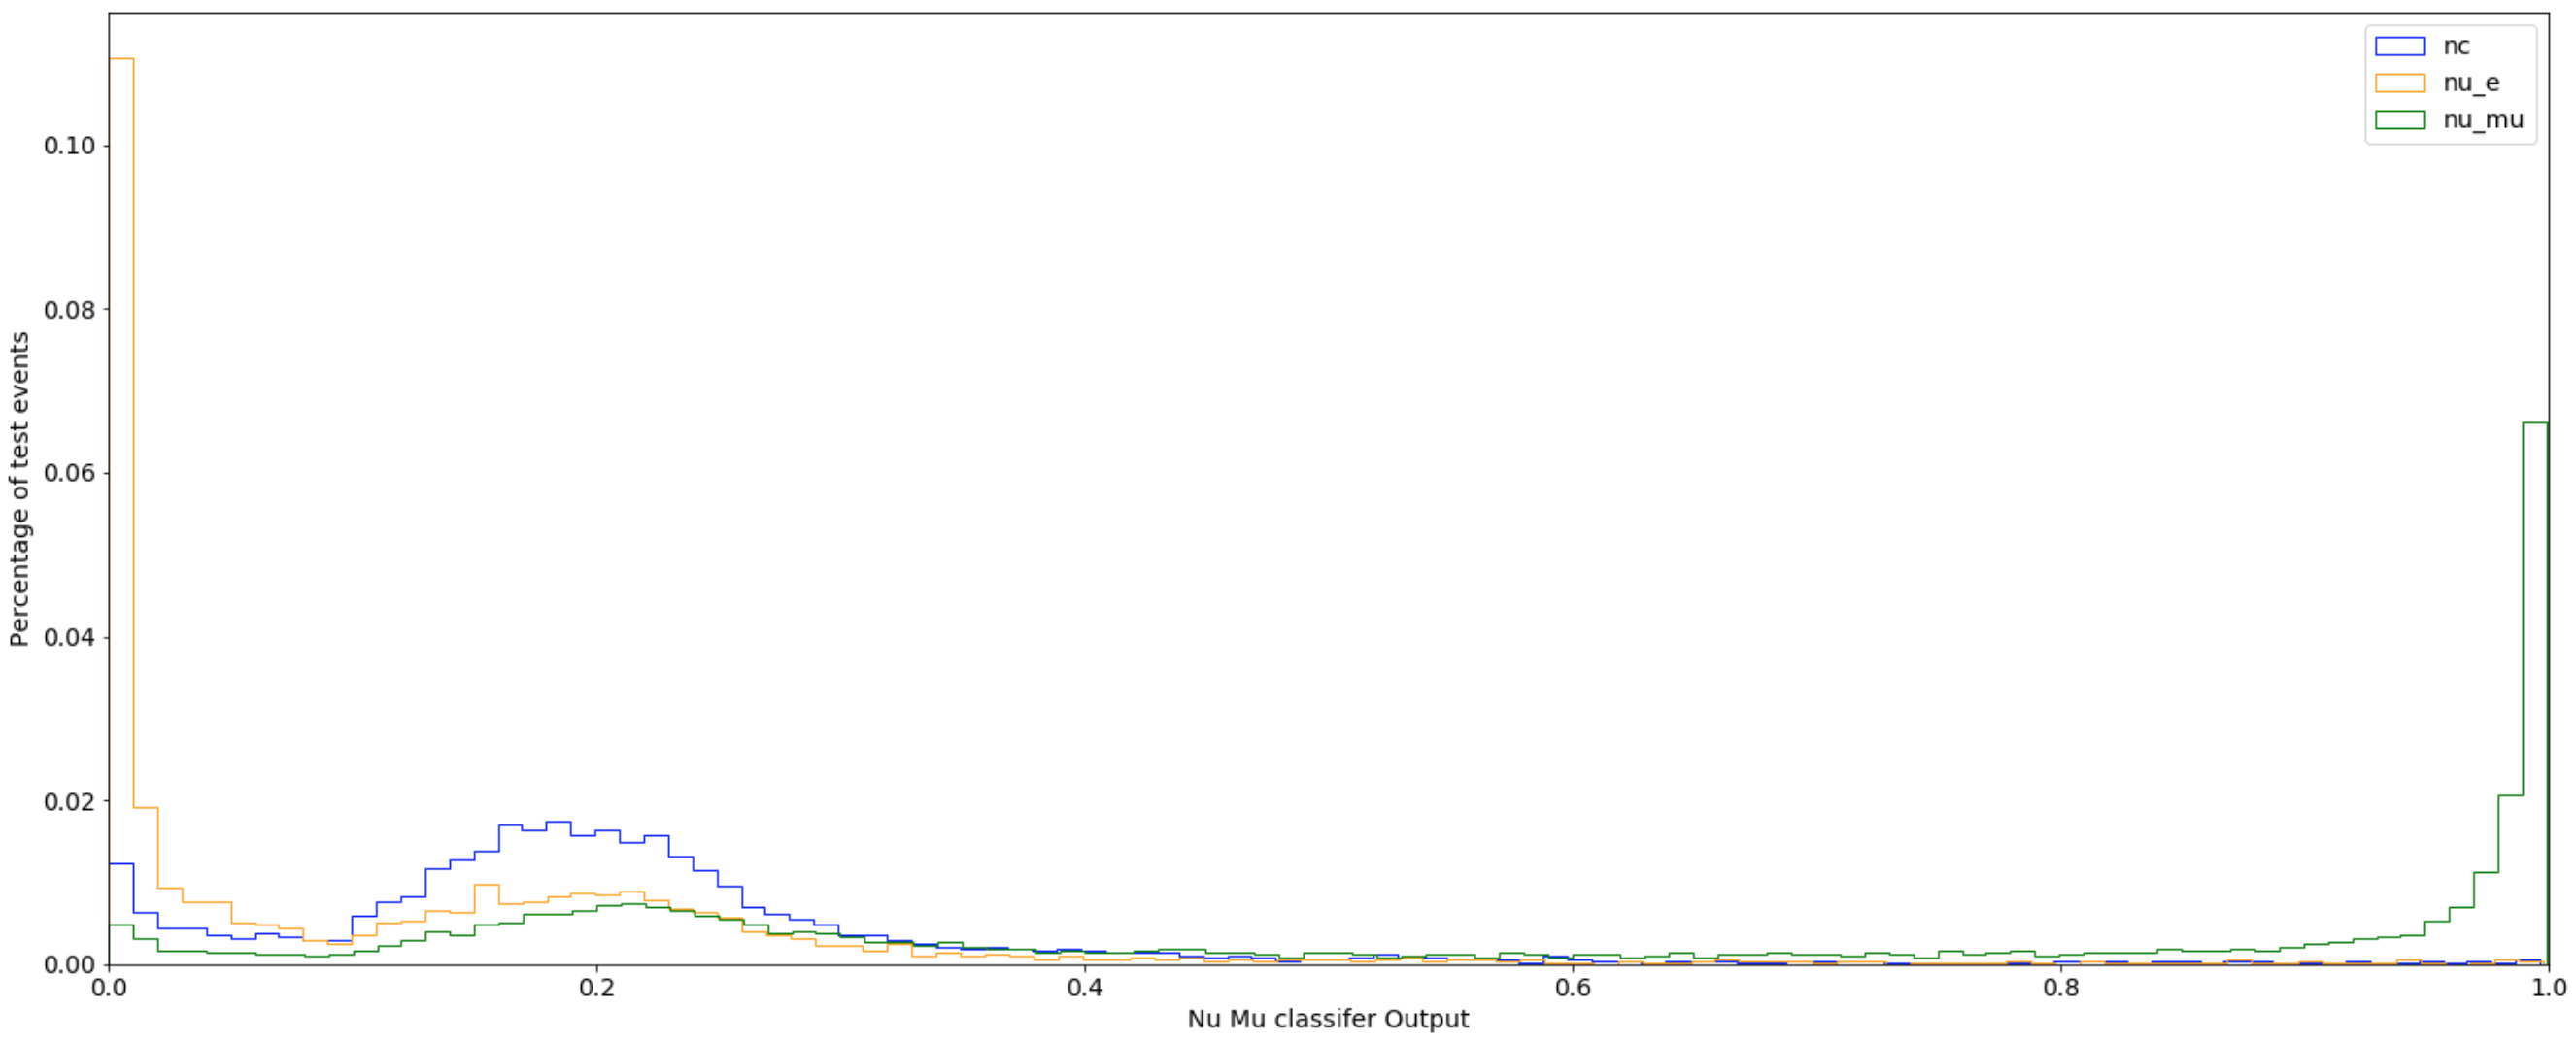
\includegraphics[width=160mm]{genie/gibuu/numu.png}
 \textbf{Figure 17.} \textit{$\nu_\mu$ classification output histogram. The dataset was trained using balanced GENIE only events- the same training process as the model in figures 13 and 14, but was evaluated on a balanced GiBUU dataset. Figures show the probability of being classified a $\nu_\mu$ for events of all the interaction types.}

 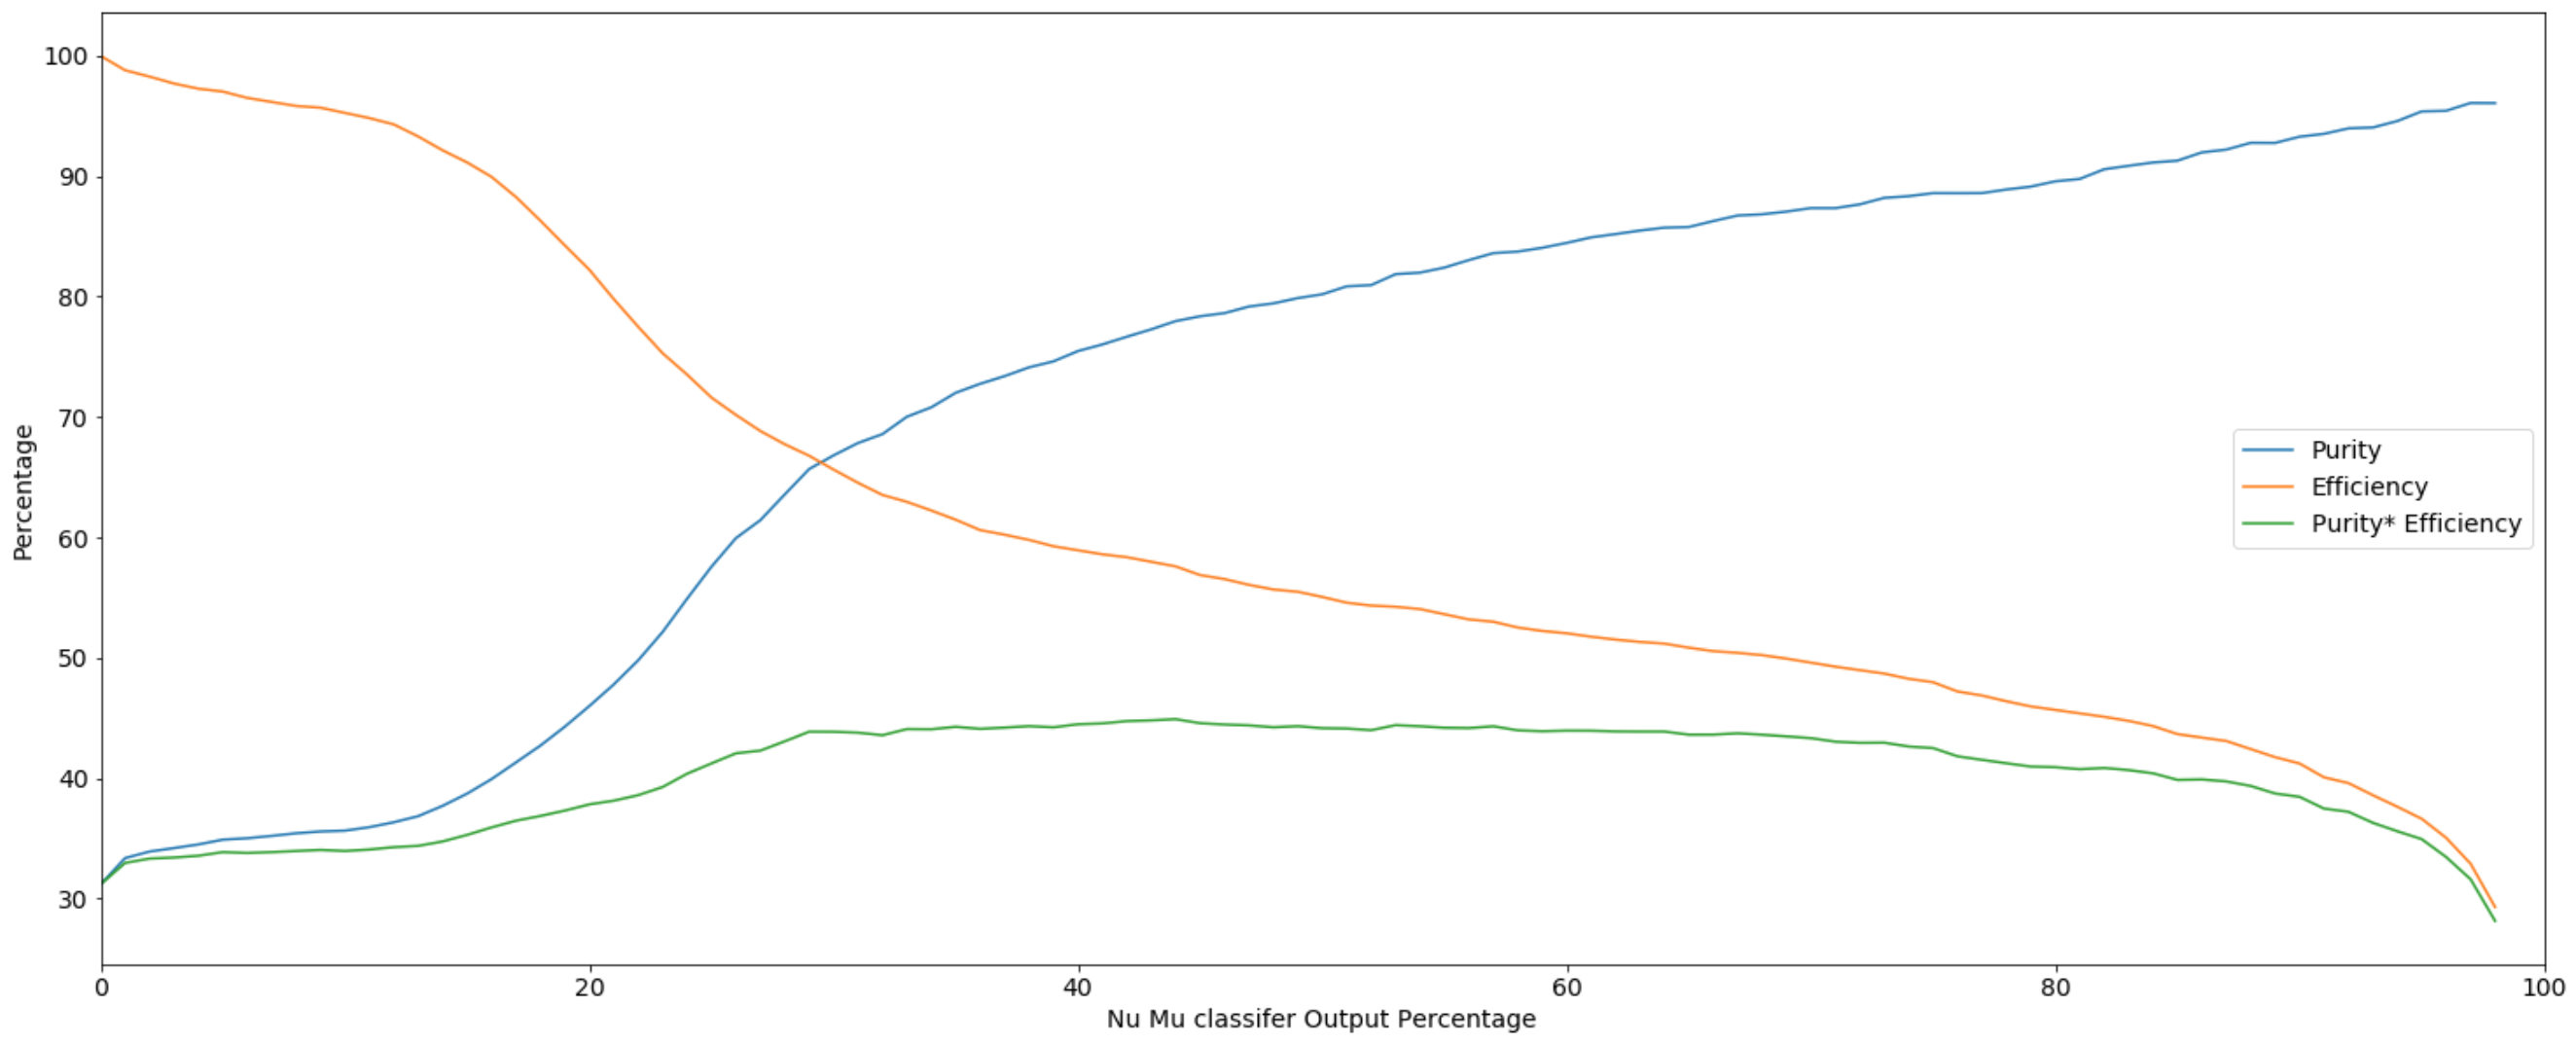
\includegraphics[width=160mm]{genie/gibuu/numupe.png}
 \textbf{Figure 18.} \textit{$\nu_e$ classification output histogram. The dataset was trained using balanced GENIE only events- the same training process as the model in figures 13 and 14, but was evaluated on a balanced GiBUU dataset. Figures show the probability of being classified a $\nu_e$ for events of all the interaction types.}
\end{figure}

\noindent The classifier was tested on 8856 events produced by GiBUU with an equal number of each of the interaction types. The $\nu_\mu$ classifier performs similarly when tested on GiBUU events as to when tested on GENIE events, with a similar proportion of events being correctly classified with a confidence level of above 90\%, this can be seen by comparing Figures 17 and 13. The difference between the two classification results is that at at confidence levels between 10\% and 30\%, see Figure 17, all three event types can be seen to be classified with similar confidence levels by the model with a similar distribution. Due to this mis-classification of $\nu_\mu$ events, the efficiency curve in Figure 18 falls steeply over this model output range, but then flattens out, as very few events are classified with a confidence between 30 and 80\%. This may be because the GiBUU generator produces a class of each event that look similar to the others. This is unusual as we would expect some $\nu_\mu$ and $NC$ events to look similar, and some $\nu_e$ and $NC$ events to look similar, but not $\nu_\mu$ and $\nu_e$ events to do so. \medskip

\begin{figure}[t!]
 \centering
 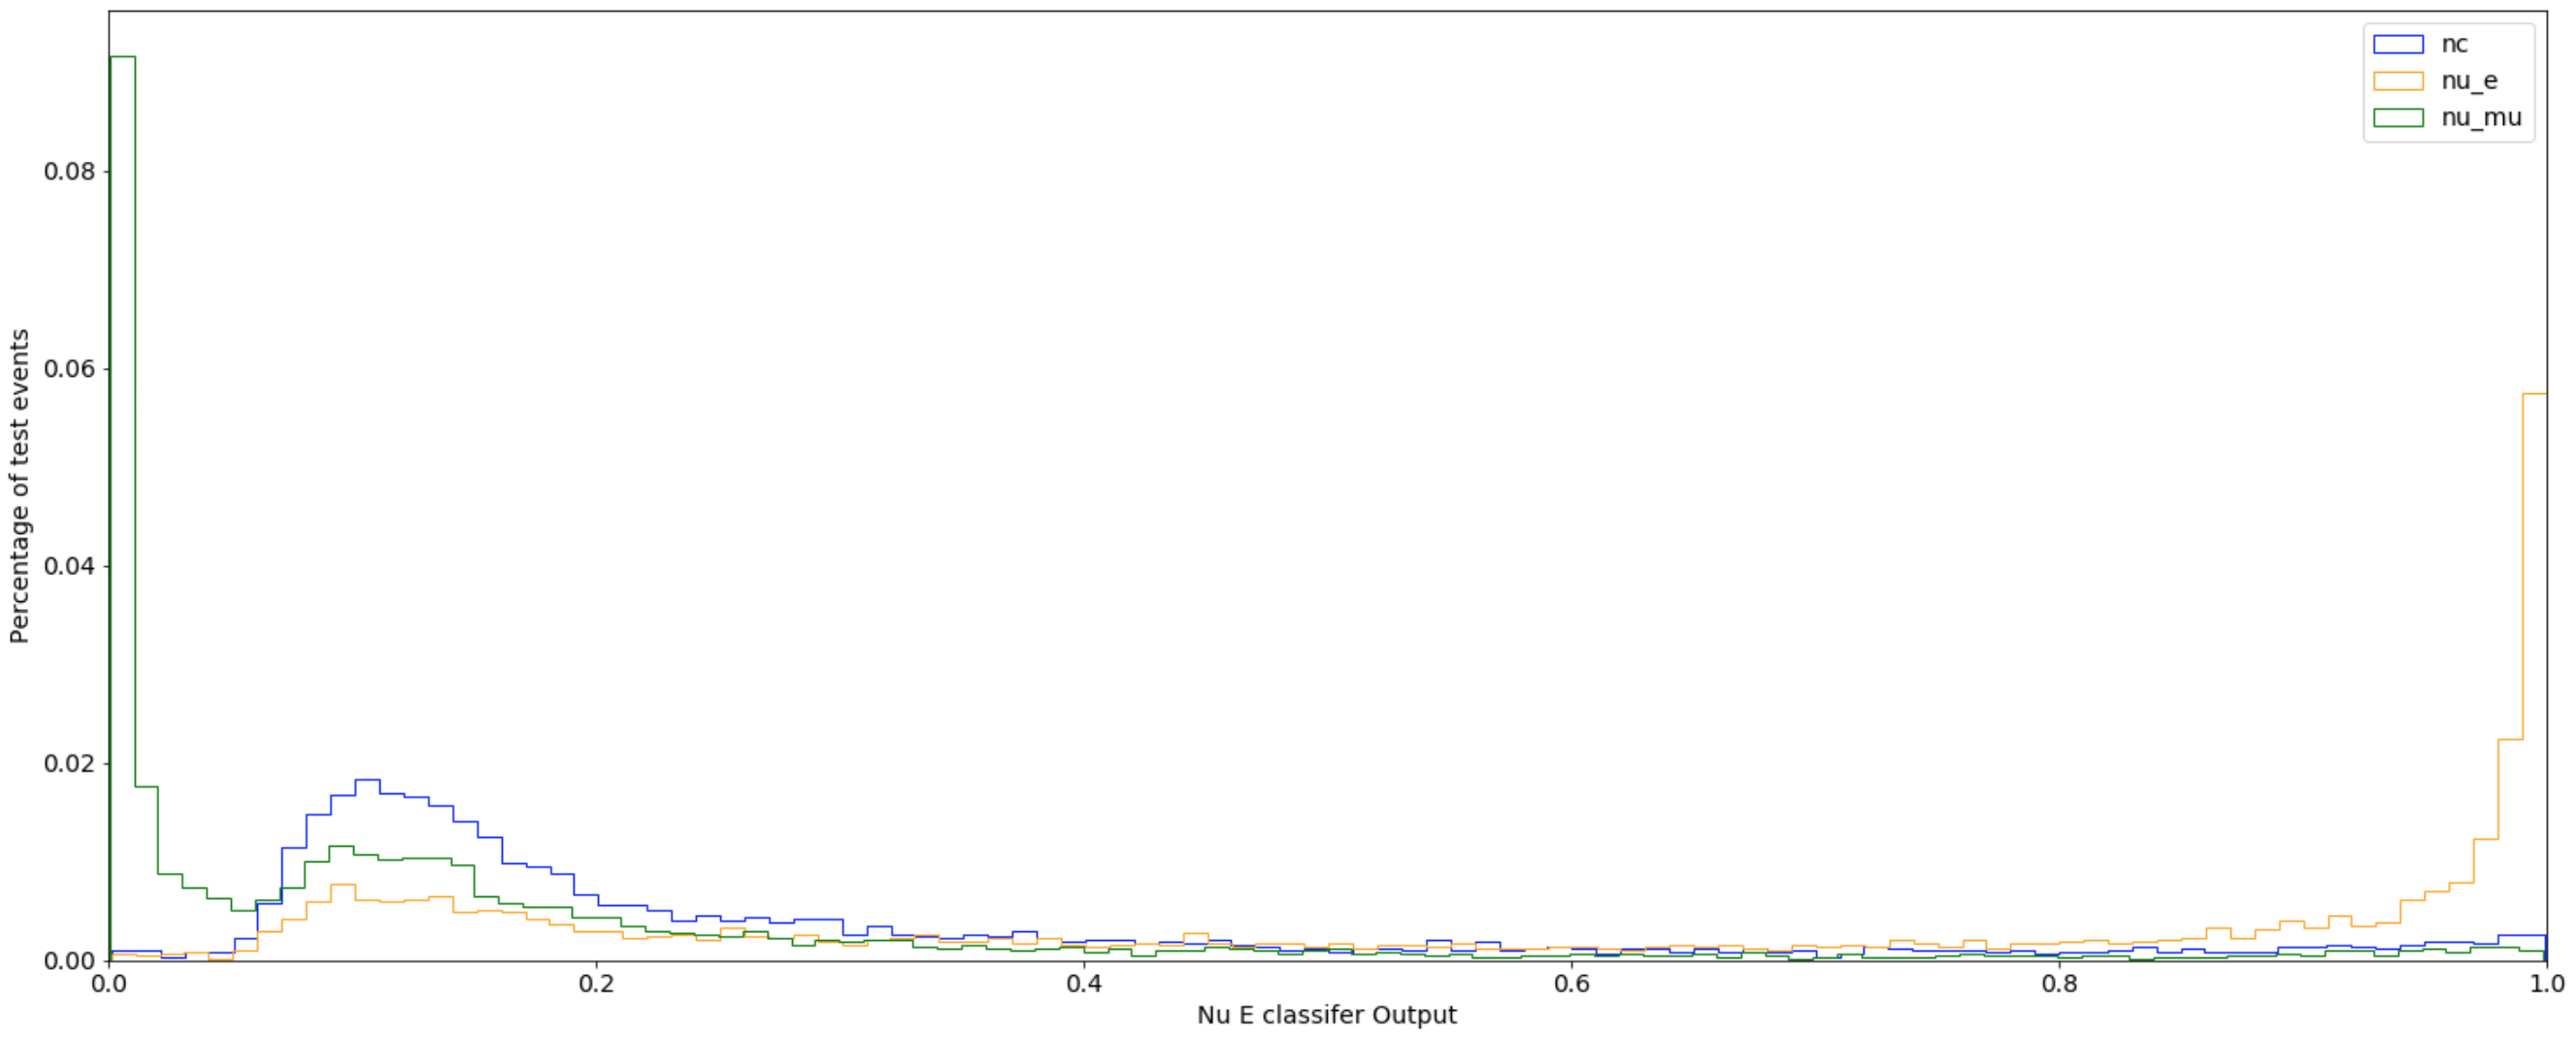
\includegraphics[width=160mm]{genie/gibuu/nue.png}
 \textbf{Figure 19.} \textit{Purity, efficiency and their product, curves for the $\nu_\mu$ classifier trained on a balanced GENIE dataset and tested on a balanced GiBUU dataset. The x-axis shows the confidence percentage of the network out (output multiplied by 100 to give the percentage).}

 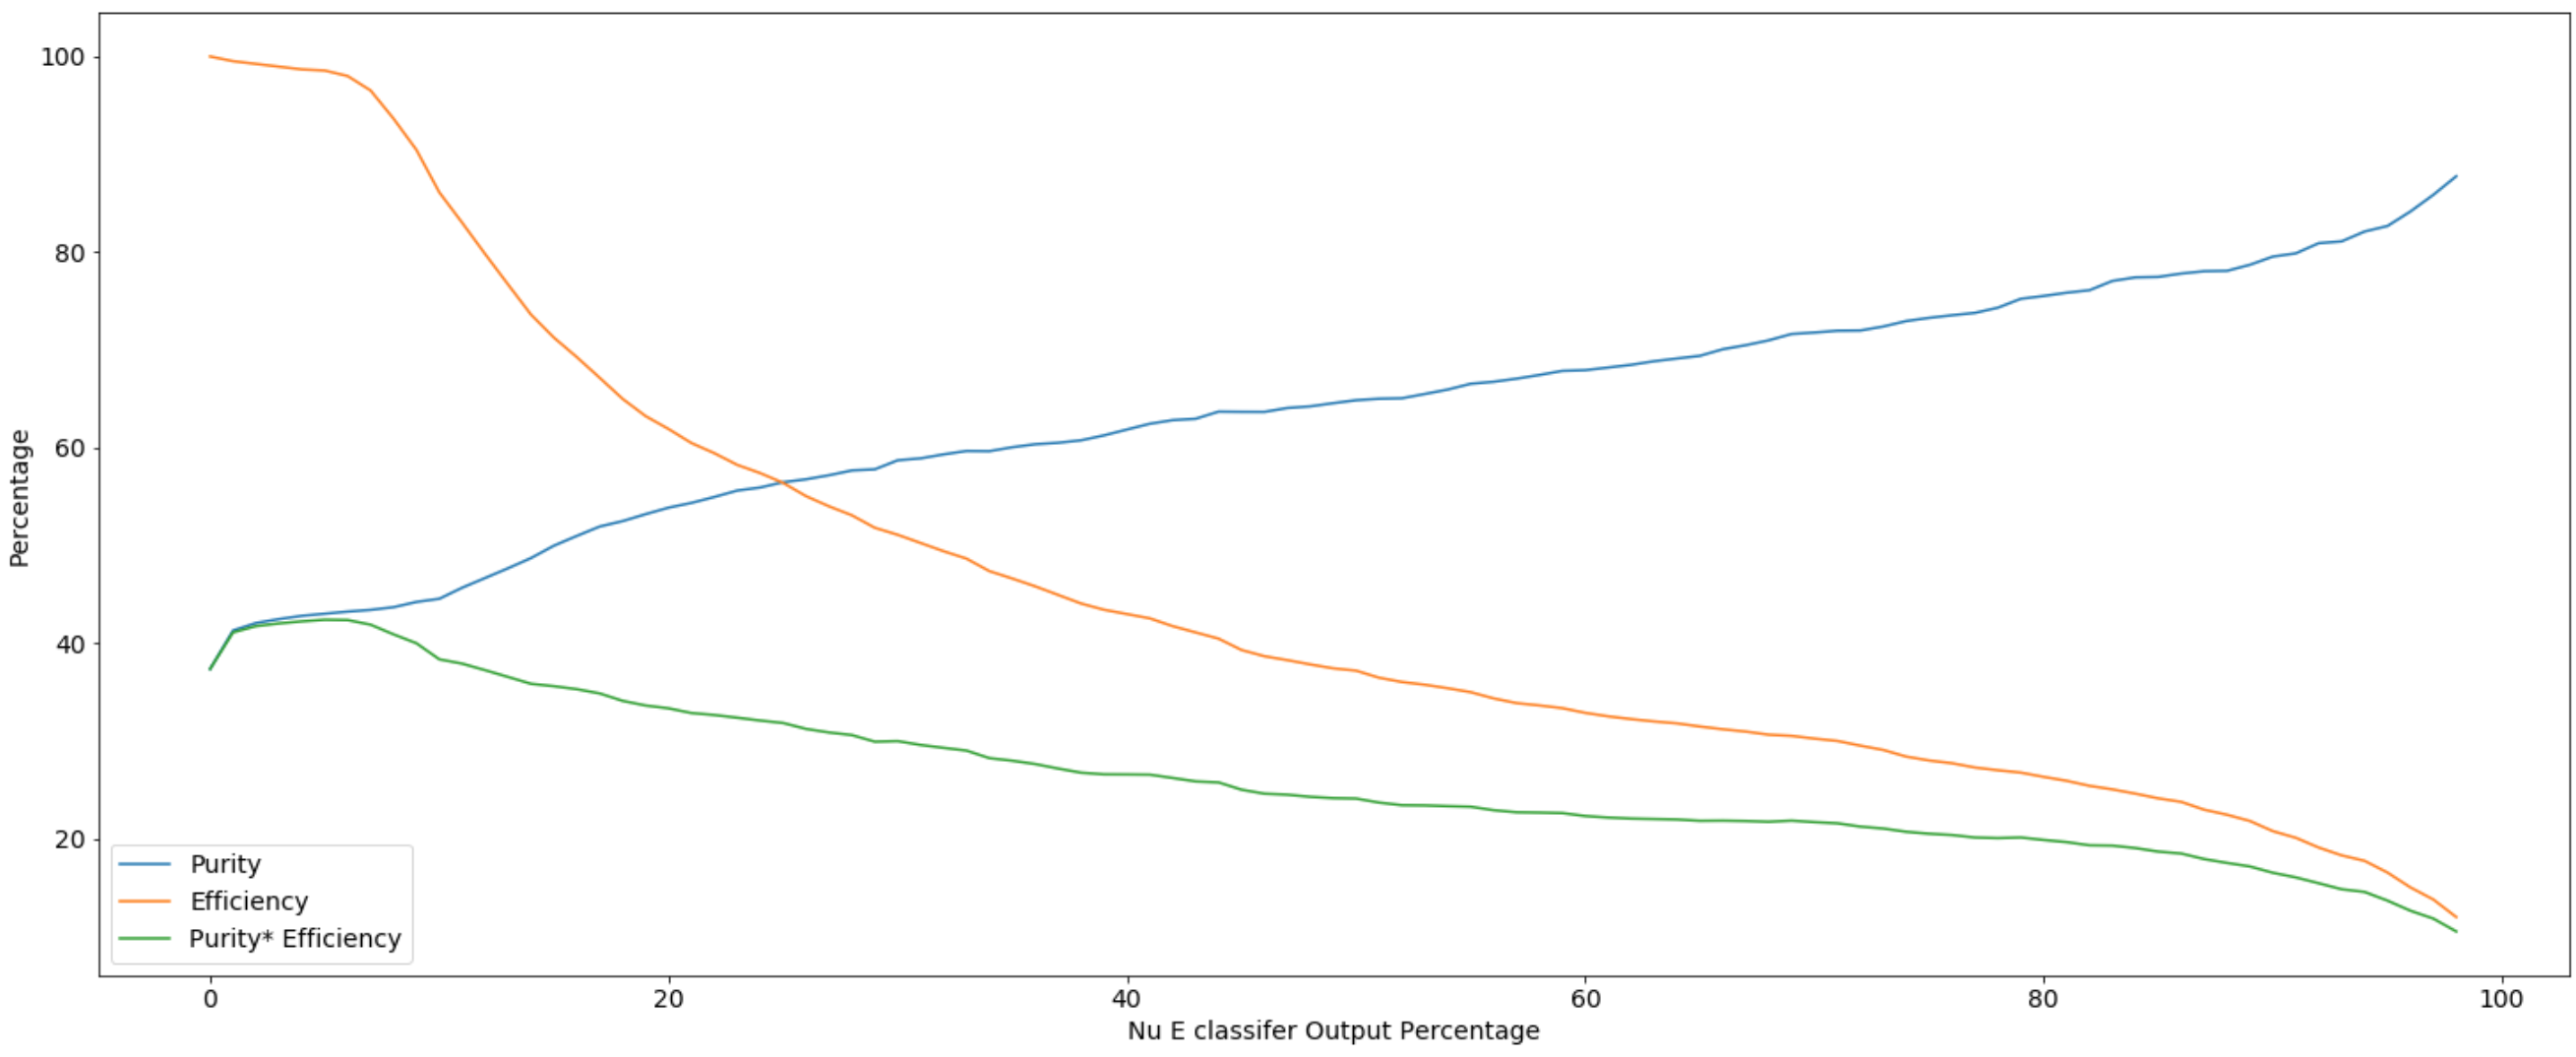
\includegraphics[width=160mm]{genie/gibuu/nuepe.png}
 \textbf{Figure 20.} \textit{Purity, efficiency and their product, curves for the $\nu_e$ classifier trained on a balanced GENIE dataset and tested on a balanced GiBUU dataset.}
\end{figure}

\noindent Looking at the classification of the $\nu_e$ events produced by GiBUU in Figure 19, we see that the model is not as strong in classifying events produced by GiBUU compared to produced by GENIE for the GENIE trained model. A similar proportion of the event samples were confidently correctly classified as $\nu_e$ events with a confidence of 90\% and above. The model also correctly classifies $\nu_\mu$ events as not $\nu_e$ with a high level of confidence, however the proportion of such events is smaller in the GiBUU dataset than the GENIE testing dataset. A reason for this is likely the slightly lower confidence classification of $\nu_\mu$ events, as well as $NC$ and $\nu_e$ events between 5\% and 25\% confidence levels. As with the $\nu_\mu$ classifier, the similarity in the distribution of confidence levels for the three interaction types in this confidence range is very similar, and indicates some similarity that the model is unable to discern between these events. As there are a larger number of $\nu_e$ events are wrongly classified with a high confidence, the efficiency curve in Figure 20 falls very steeply, resulting in a poor purity efficiency product curve compared to Figure 16. \medskip